\section{Results}

\subsection{Distinctiveness}

\begin{figure*}[t]
\centerline{% 
		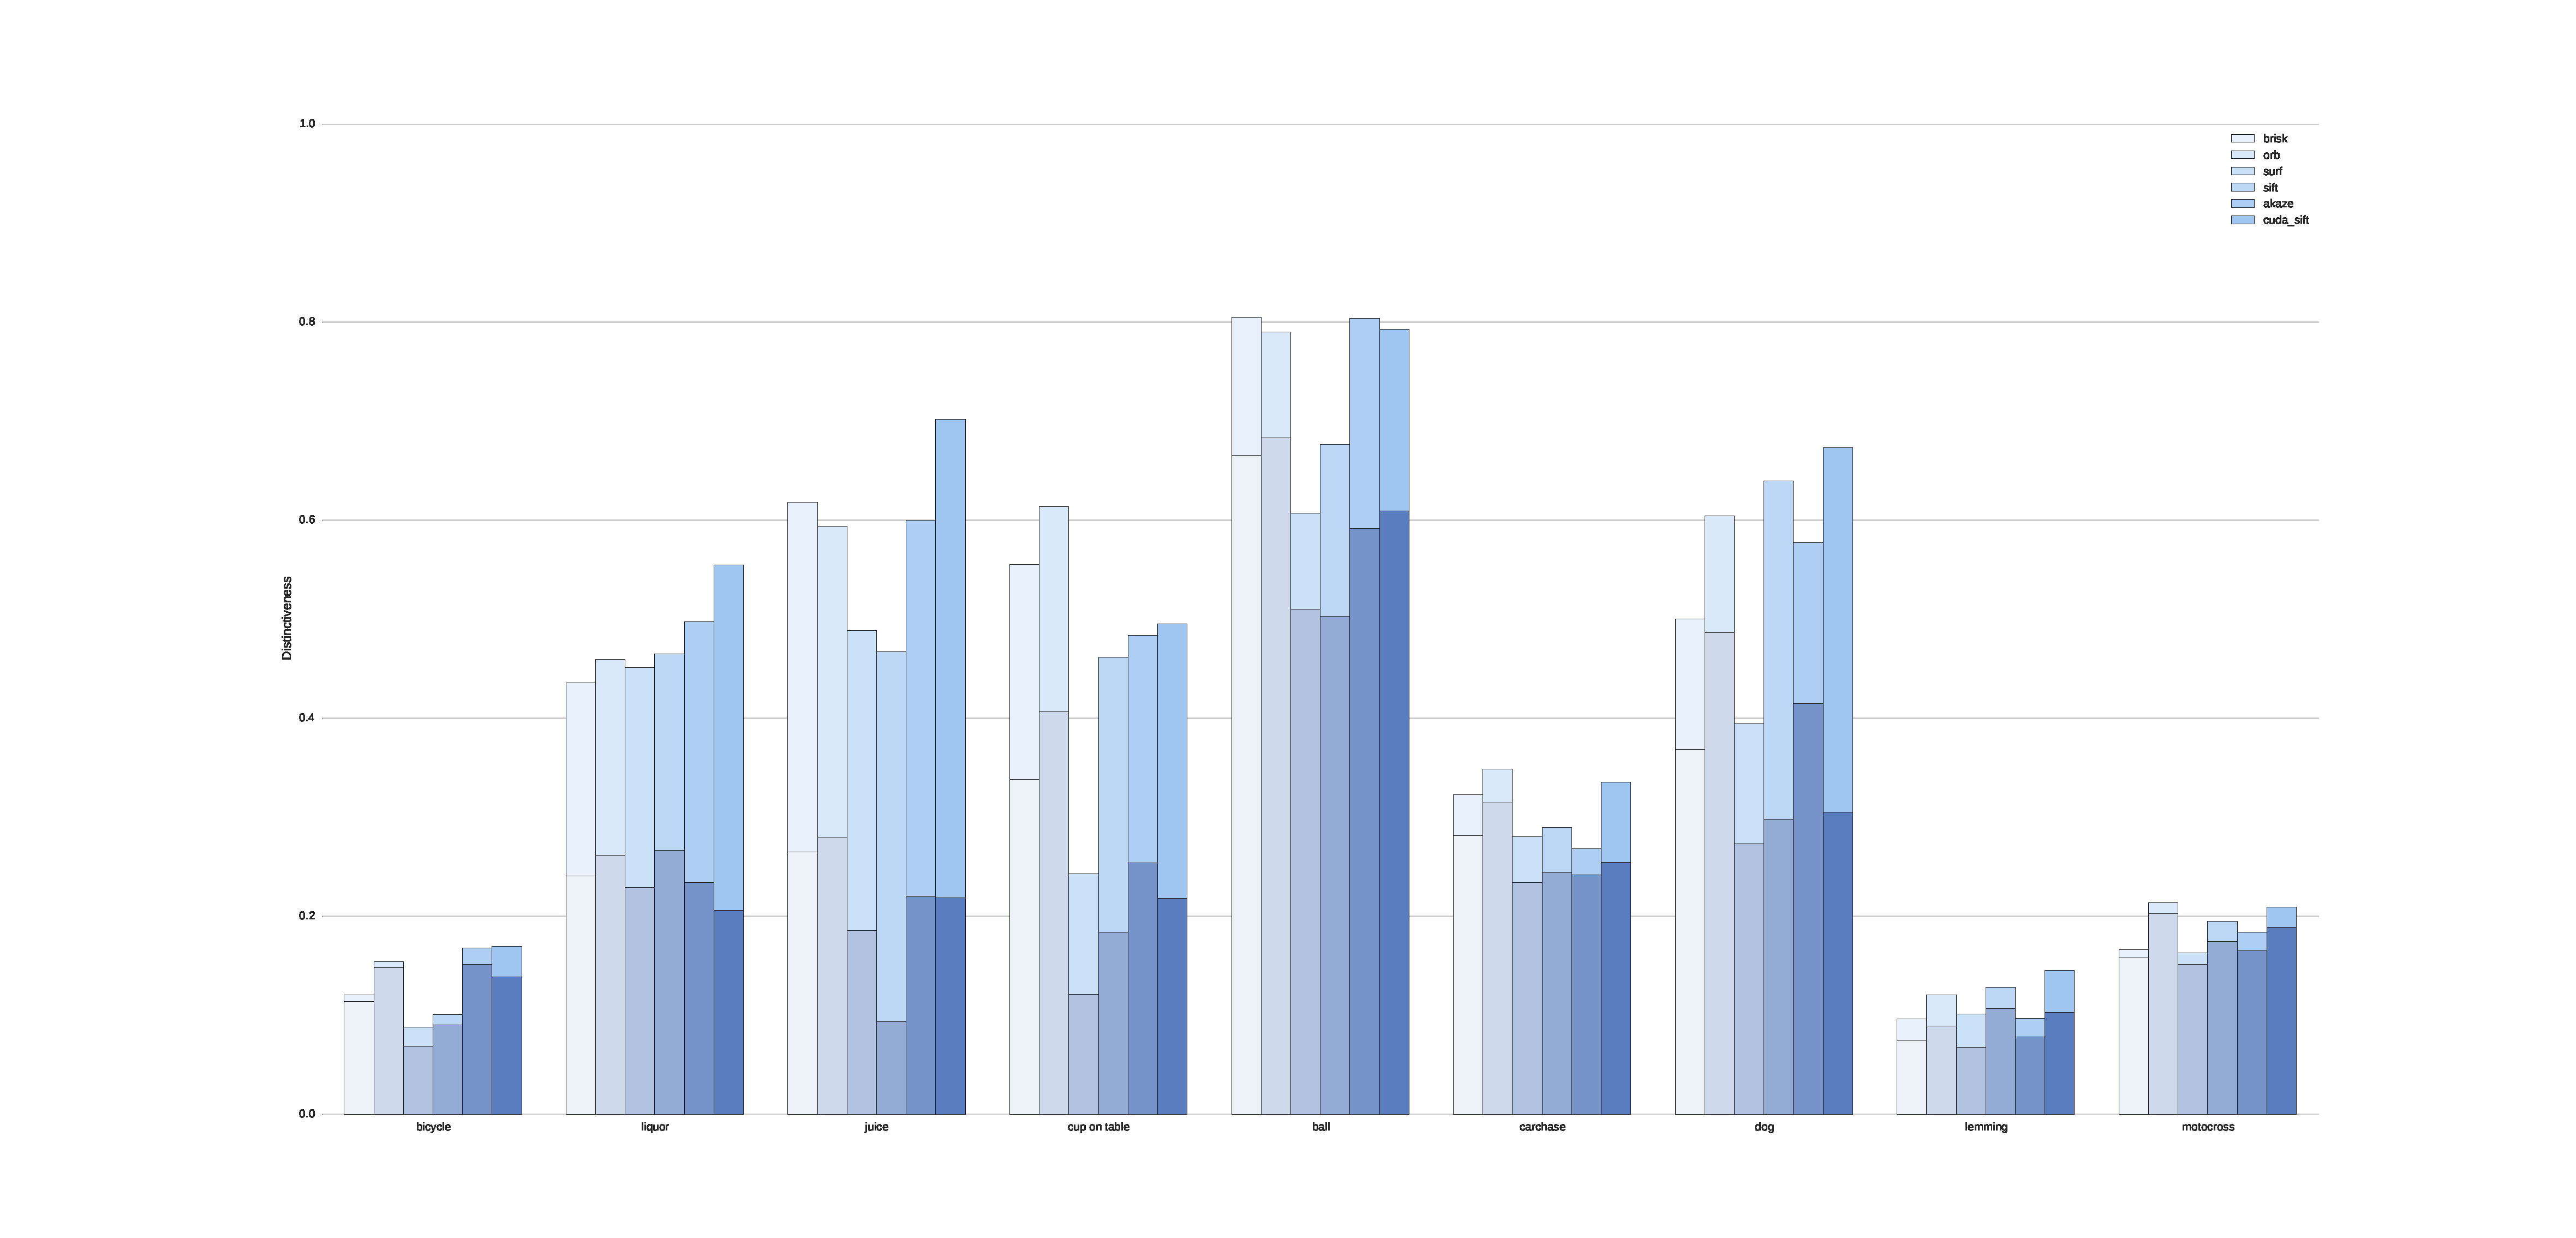
\includegraphics[width=0.98\linewidth]{imgs/distinctivenessTP.pdf}}
    \vspace{-2mm} 
	\caption{Examples taken from the dataset showing the ratio of true positives and ambiguous true positives. The lighter color bars show the number of true positives that will actually pass the second best result test.}
	\label{fig:distinctiveness}
\end{figure*}

Fig.~\ref{fig:distinctiveness} shows the amount of true positives and ambiguous true positives for a subset of the videos present in the dataset. the lighter color bars show the number of descriptors that will pass the second best ratio filter. In Tab.~\ref{table:tp_ratio} shows the average ratios of effective true positives and total number of descriptors extracted on all the dataset. By effective true positive we intend all the positives matches that pass the second best match filter. Looking at the statistics it is interesting to notice that BRISK and ORB extract a higher number of feature descriptors in general and Fig.~\ref{fig:distinctiveness} shows that they have also a higher number of true positives, however if we calculate the number of true positives that pass the second best match check, then cuda SIFT and AKAZE have a better ratio of effective true positives. This is an indication that those descriptors are more distinctive. Upon inspection, the number of false positives is comparable as shown in Fig.~\ref{fig:false_positives}.

\begin{table}[h]
\centerline{% 
		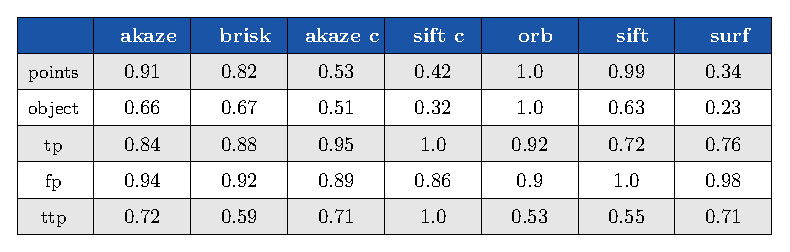
\includegraphics[width=0.98\linewidth]{tables/descriptivness_ratio.pdf}}
    \vspace{-2mm} 
	\caption{Average number of effective true positives and total feature extracted.}
	\label{table:tp_ratio}
\end{table}

\subsection{Tracking accuracy}

\begin{figure}[t]
	\vspace{2mm}
\centerline{%
	\subfigure{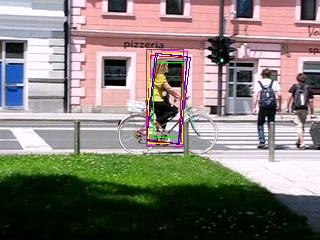
\includegraphics[width=0.48\linewidth]{imgs/results/ex1.png}}
	\subfigure{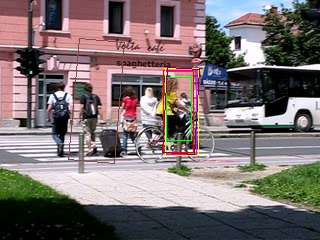
\includegraphics[width=0.48\linewidth]{imgs/results/ex2.png}}}
	\vspace{-2mm}
\centerline{%
	\subfigure{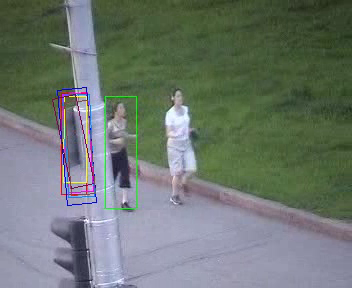
\includegraphics[width=0.48\linewidth]{imgs/results/ex5.png}}
	\subfigure{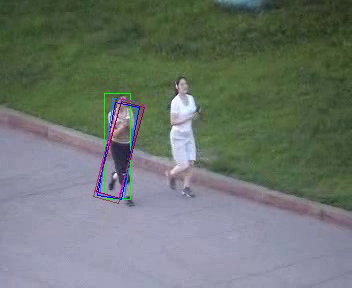
\includegraphics[width=0.48\linewidth]{imgs/results/ex6.png}}}
\caption{Examples showing the behaviour of the feature descriptors upon occlusion. Upon recovery from track loss more descriptive descriptors allow the tracker to recover faster.}
\vspace{-3mm}
\label{fig:tracking_results}
\end{figure}

\begin{figure}[t]
	\vspace{2mm}
\centerline{%
	\subfigure{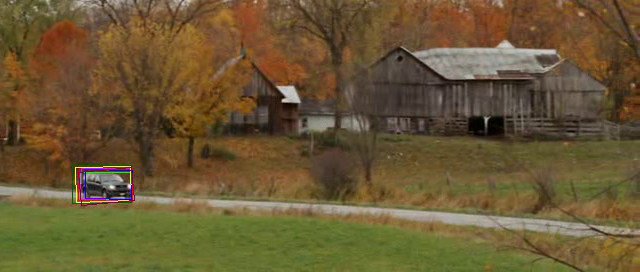
\includegraphics[width=0.48\linewidth]{imgs/results/ex3.png}}
	\subfigure{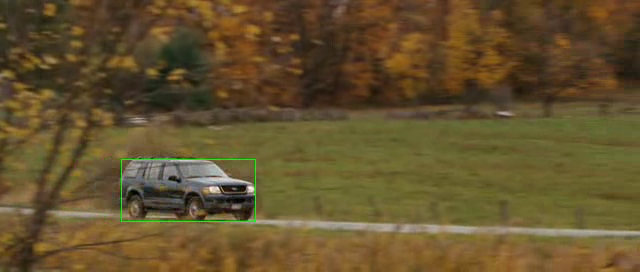
\includegraphics[width=0.48\linewidth]{imgs/results/ex4.png}}}
	\vspace{-2mm}
\caption{Despite most of the descriptors are scale invariant this example shows their weakness in working with drastic scale change.}
\vspace{-3mm}
\label{fig:tracking_results_scale}
\end{figure}

As explained in the previous section \ref{sec:accuracy}, we evaluated the performance of the feature descriptors running our tracker and calculating the overlap measure for low, medium and high accuracy requirements. It can be noticed in our results (table~\ref{table:taccuracy}) that AKAZE performs better overall, ORB BRISK and cuda SIFT have comparable results. Even if BRISK and ORB has been proven to be less descriptive, the higher amount of weak descriptors extracted seems to compensate the weaker descriptor. This is confirmed by the result of the high tracking requirements were more descriptive features such as AKAZE and cuda SIFT performs better than BRISK and ORB. It has to be noticed that an higher number of feature descriptors has an impact on the performance of the feature extraction and matching step since they are strictly correlated to the number of feature descriptors. 

\subsection{Tracking performance}

We evaluate the performance of each feature descriptor in three different steps: detection, computation and matching. Fig.~\ref{fig:speed} shows the overall results on the dataset. It is interesting to notice that despite AKAZE exploits multiple core on the CPU, its detection part is expensive due to the non-linear filtering. Brisk and ORB are faster but then the matching step is more expensive given the higher number of features extracted. Please note that this numbers are only informative. We think that it is not fair to compare multi-threaded implementations (e.g AKAZE) with single threaded (SIFT) or GPU implementation (SIFT).

\begin{figure}
	%\vspace{-2mm}
	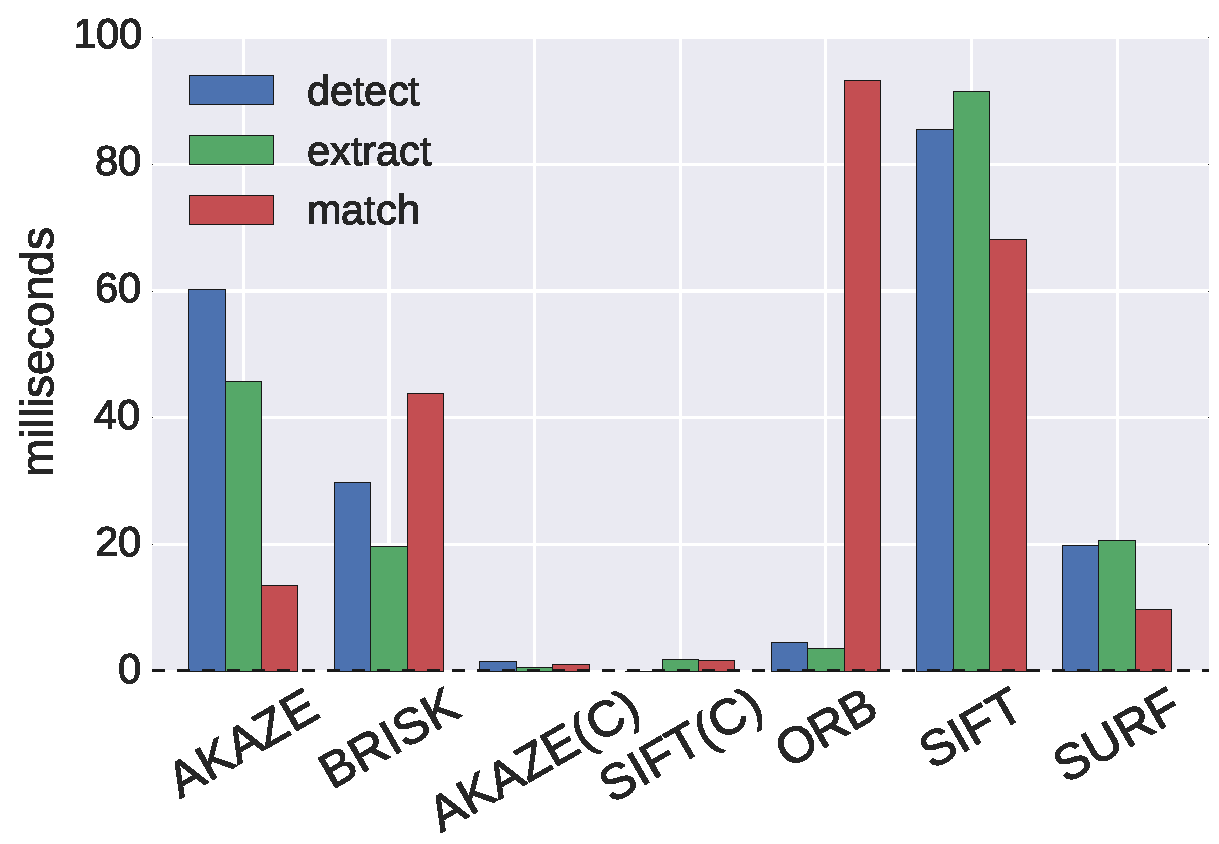
\includegraphics[width=0.95\linewidth]{imgs/performances.pdf}
\vspace{-2.5mm}	
\caption{Performance of the compute,detect and match steps of each feature descriptor.}
\label{fig:speed}
\end{figure}

\begin{table}
\caption{Average time spent on a single frame by the tracker.}
	%\vspace{-2mm}
	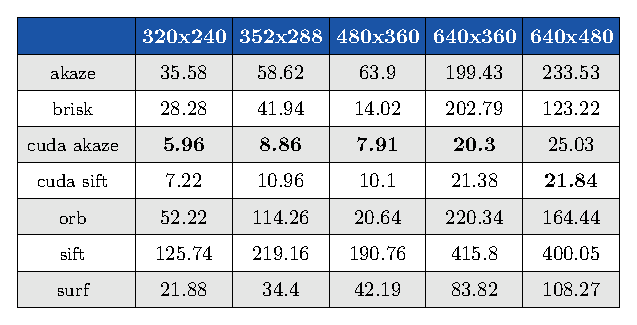
\includegraphics[width=0.95\linewidth]{tables/resolution_times.pdf}
\vspace{-2.5mm}	
\label{fig:fps}
\end{table}

\begin{figure}
	%\vspace{-2mm}
	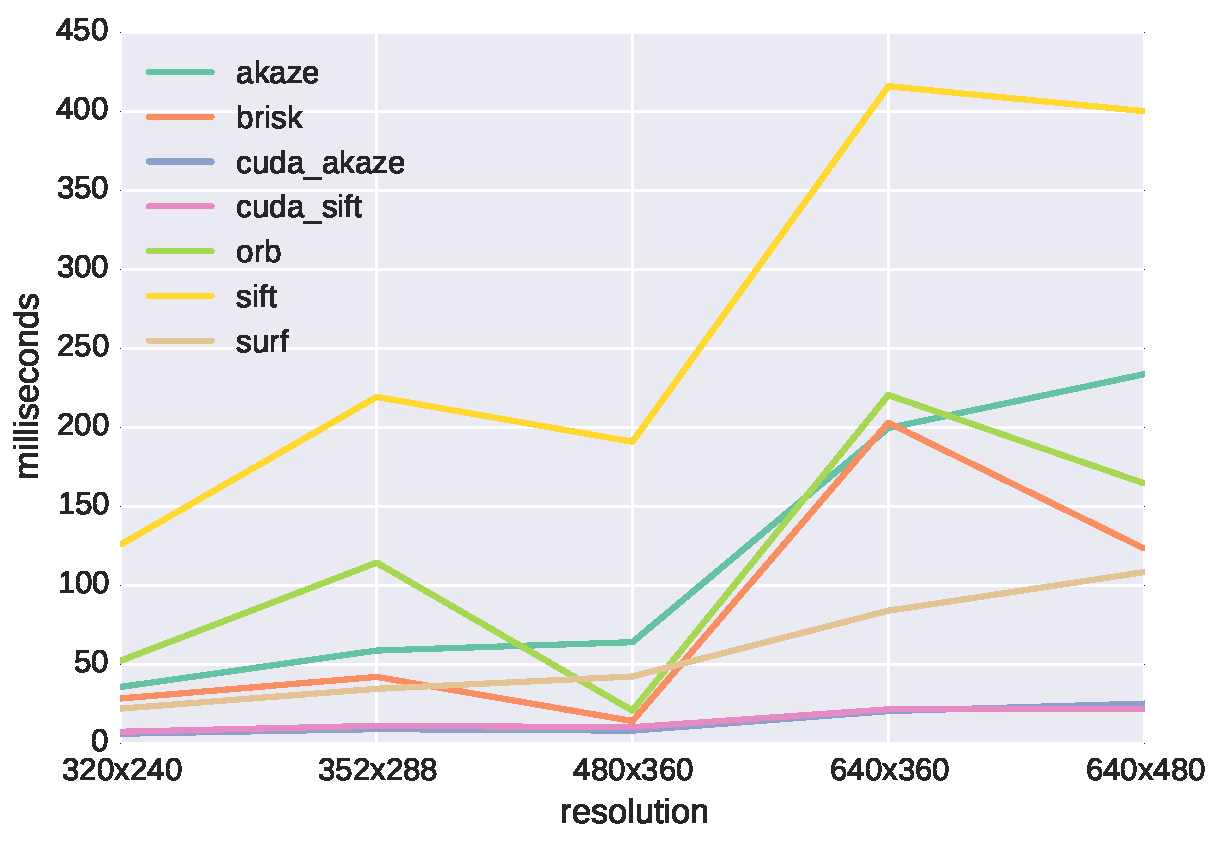
\includegraphics[width=0.95\linewidth]{imgs/tracker_fps.pdf}
\vspace{-2.5mm}	
\caption{Performance of the compute,detect and match steps of each feature descriptor.}
\label{fig:speed}
\end{figure}



\begin{table*}[h]
\centerline{% 
		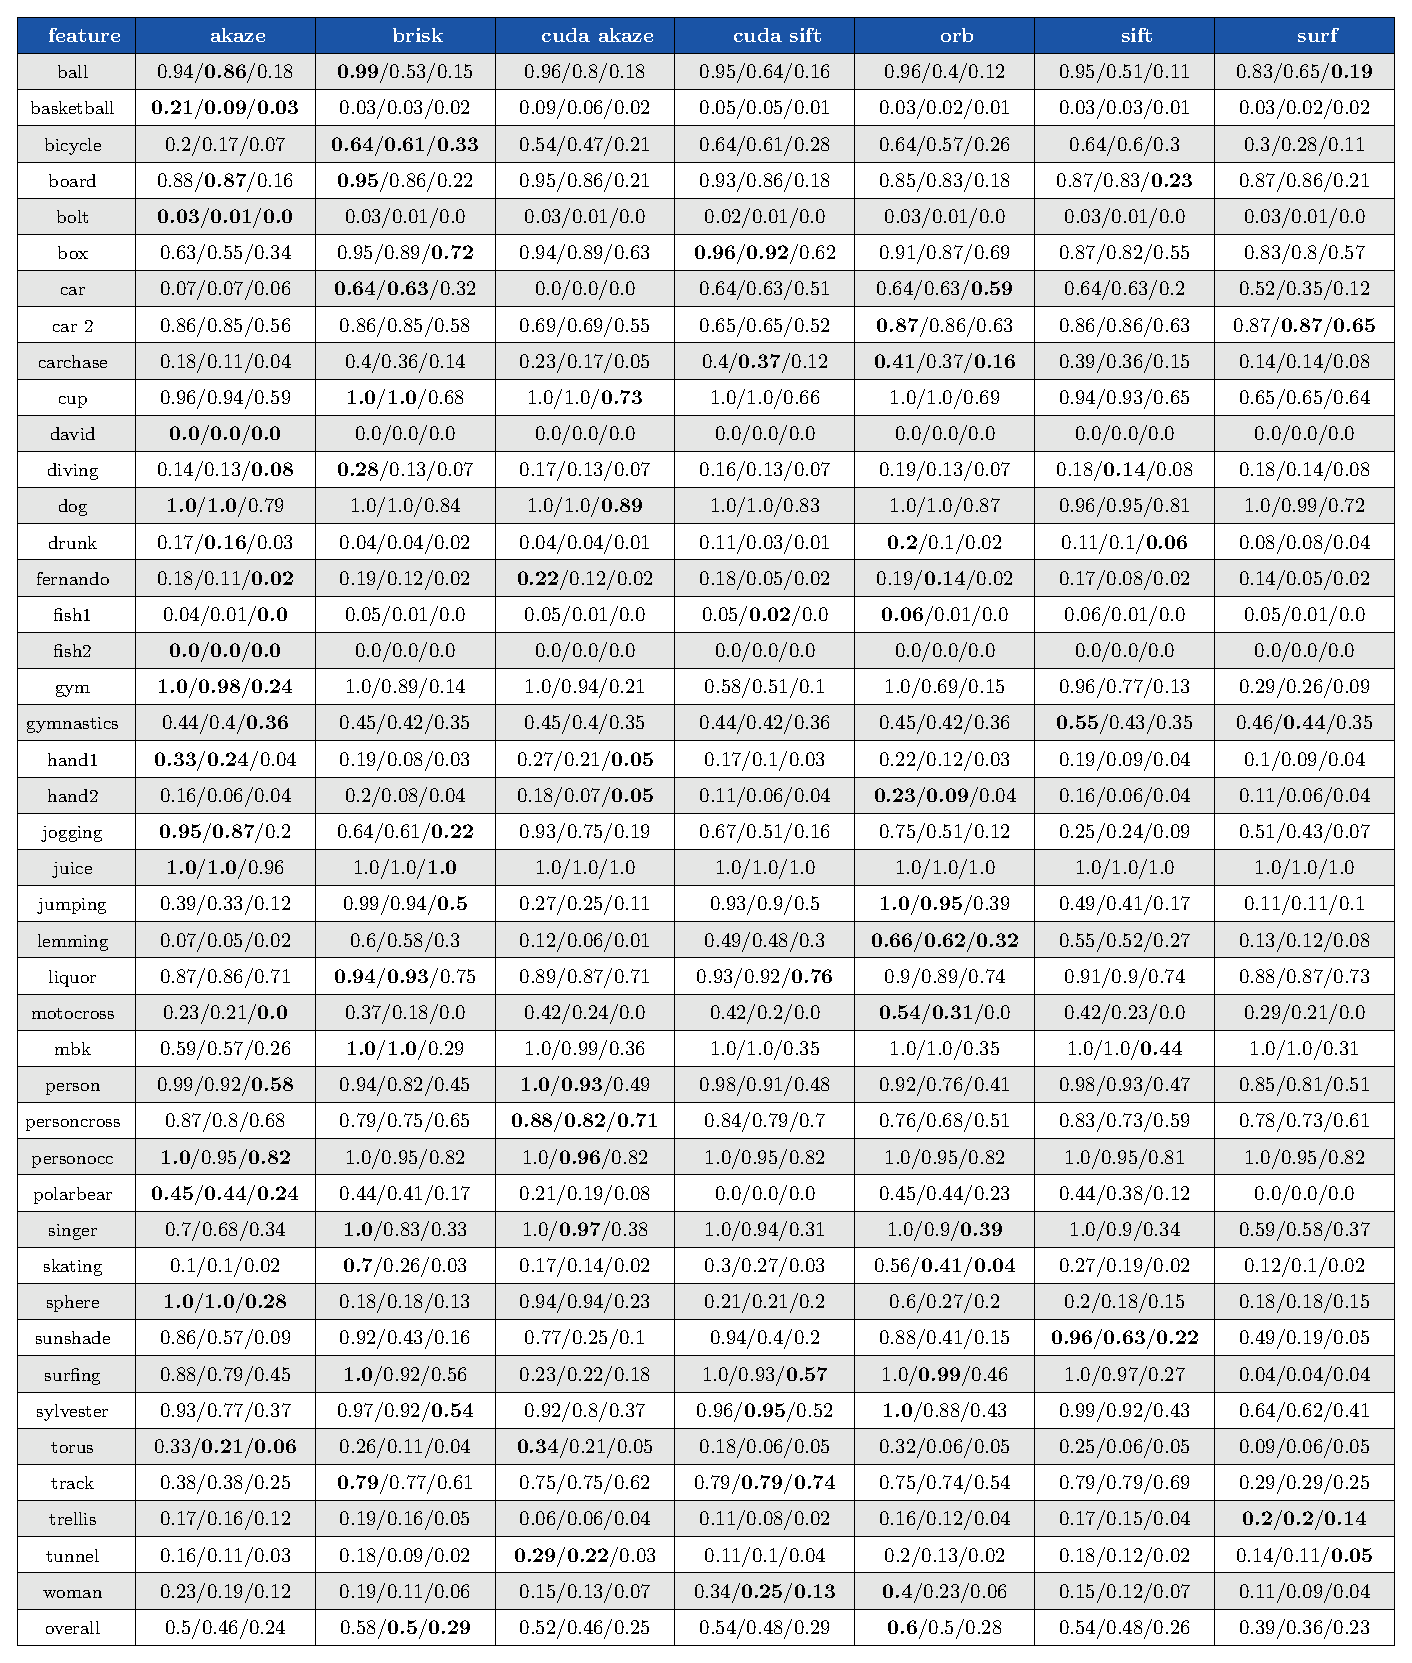
\includegraphics[width=0.98\linewidth]{tables/tracking_precision.pdf}}
    \vspace{-2mm} 
	\caption{Tracking results with low,medium and high accuracy requirements. Akaze performs better overall.}
	\label{table:taccuracy}
\end{table*}